\lstset{
  basicstyle=\ttfamily,
  columns=fullflexible,
  frame=single,
  breaklines=true,
  postbreak=\mbox{\textcolor{red}{$\hookrightarrow$}\space},
}
\chapter{Implementasi dan Pengujian}
\label{chap:implementasiDanPengujian}
\setcounter{secnumdepth}{3}

\section{Implementasi}
\subsubsection{Lingkungan Pengembangan dan Pengujian Fungsional}
\paragraph{} Pembangunan perangkat lunak ini memakai bahasa pemrogaraman server PHP 5 dan MySQL 5.0 sebagai basis datanya. Pengembangan perangkat lunak ini dilakukan di komputer dengan spesifikasi perangkat keras dan perangkat lunaknya sebagai berikut:
\begin{itemize}
\item \textbf{Perangkat Keras}
\begin{enumerate}
	\item Prosesor AMD A6 VISION
	\item RAM 4 GB
	\item 500 GB harddisk
	\item Monitor
	\item Keyboard
	\item Mouse
\end{enumerate}
\item \textbf{Perangkat Lunak}
\begin{enumerate}
	\item Sistem Operasi Windows 8
	\item NetBeans IDE 8.0.2
	\item Server phpMyAdmin 4.3.11
	\item XAMPP Control Panel v3.2.1
	\item Client: Google Chrome 61.0.3163.100 32-bit
	\item Microsoft Excel 2015
\end{enumerate}

\end{itemize}
\subsection{Implementasi Basis Data}
\paragraph{}Implementasi basis data dalam Aplikasi Pembangkit Jadwal Dosen menggunakan satu tabel basis data. Tabel tersebut adalah tabel jadwal\_dosen yang menyimpan informasi-informasi seperti:
\begin{enumerate}
	\item user yang memiliki jadwal terkait
	\item hari berlangsungnya jadwal
	\item jam dimulainya kegiatan jadwal 
	\item durasi (dalam jam) lama berlangsungya jadwal
	\item nama kegiatan jadwal
	\item waktu terakhir jadwal diupdate
\end{enumerate}

\subsection{Implementasi Kelas}
Implementasi kelas dalam Aplikasi Pembangkit Jadwal Dosen terdiri dari kelas - kelas sebagai berikut:
\begin{enumerate}
	\item Kelas \textit{controller} EntriJadwalDosen\\
	Merupakan kelas yang mengatur hubungan antara kelas view EntriJadwalDosen dan kelas model JadwalDosen\_model.
	\item Kelas \textit{controller} LihatJadwalDosen\\
	Merupakan kelas yang berfungsi menghubungkan antara kelas view LihatJadwalDosen dan kelas model JadwalDosen\_model.
	\item Kelas \textit{view} EntriJadwalDosen yang berfungsi membuat \textit{user interface} untuk memasukan jadwal
	\item Kelas \textit{view} LihatJadwalDosen yang berfungsi membuat \textit{user interface} untuk memlihat jadwal
	\item Kelas model JadwalDosen\_model yang berfungsi untuk menulis atau membaca ke basis data.
\end{enumerate}

\section{Pengujian}
\paragraph{} Pengujian aplikasi ini dilakukan dengan menggunakan metode pengujian \textit{Black-Box Testing}. Pengujian ini difokuskan pada pengujian fungsional. Maksud dari pengujian fungsional ini adalah untuk menguji reaksi perangkat lunak terhadap aksi yang dilakukan oleh pengguna. Bila reaksi sistem tidak sesuai yang diharapkan, maka aplikasi masih memilki kekurangan.

\subsection{Pengujian Fungsional}
\subsubsection{Pengujian Fungsional Login}
Hasil pengujian dapat dilihat pada Tabel 5.1
\begin{center}
	\begin{table}[H]
		\begin{tabular}{|p{5cm}|p{5cm}|p{5cm}|}
		\hline
		\centering Aksi	& 	\centering Reaksi yang diharapkan &  \multicolumn{1}{c|}{Reaksi PL} \\
		\hline
		Menekan tombol login & Menampilkan menu login & Menampilkan menu login \\
		\hline
		\end{tabular}
		\caption{Pengujian Login}
	\end{table}
\end{center}

\subsubsection{Pengujian Fungsional Entri Jadwal Dosen}
Hasil pengujian dapat dilihat pada Tabel 5.2
\begin{center}
	\begin{table}[H]
		\begin{tabular}{|p{5cm}|p{5cm}|p{5cm}|}
		\hline
		\centering Aksi	& 	\centering Reaksi yang diharapkan &  \multicolumn{1}{c|}{Reaksi PL} \\
		\hline
		Memasukan data-data yang diperlukan untuk input jadwal & Jadwal yang sudah dimasukan muncul pada halaman Entri Jadwal Dosen & Jadwal yang sudah dimasukan muncul pada halaman Entri Jadwal Dosen \\
		\hline
		Data jadwal yang dimasukan tidak lengkap & Jadwal dimasukan dengan data yang sesuai nilai \textit{default} yang ditampilkan di menu & Jadwal dimasukan dengan data yang sesuai nilai \textit{default} yang ditampilkan di menu \\
		\hline
		Waktu dimulainya jadwal baru sama dengan jadwal yang sudah pernah dimasukan sebelumnya & Menampilkan pesan kesalahan dan batal memasukan data ke dalam database & Jadwal masuk ke dalam database, namun tidak muncul di halaman Entri Jadwal Dosen maupun halaman Lihat Jadwal Dosen \\
		\hline
		\end{tabular}
		\caption{Pengujian Fungsional Entri Jadwal Dosen}
	\end{table}
\end{center}

\subsubsection{Pengujian Fungsional Edit Jadwal Dosen}
Hasil pengujian dapat dilihat pada Tabel 5.3
\begin{center}
	\begin{table}[H]
		\begin{tabular}{|p{5cm}|p{5cm}|p{5cm}|}
		\hline
		\centering Aksi	& 	\centering Reaksi yang diharapkan &  \multicolumn{1}{c|}{Reaksi PL} \\
		\hline
		Memilih jadwal yang akan diedit & Memunculkan modal yang berisi menu edit yang menampilkan data-data jadwal yang sedang dipilih tersebut. Data-data tersebut juga dapat diubah oleh pengguna sesuai kebutuhannya & Memunculkan modal yang berisi menu edit yang menampilkan data-data jadwal yang sedang dipilih tersebut. Data-data tersebut juga dapat diubah oleh pengguna sesuai kebutuhannya \\
		\hline
		Memilih tombol simpan & Modal ditutup , data jadwal di \textit{database} diupdate sesuai dengan input user dan menampilkan menu Entri Jadwal Dosen & Modal ditutup , data jadwal di \textit{database} diupdate sesuai dengan input user dan menampilkan menu Entri Jadwal \\
		\hline
		Memilih tombol keluar & Modal ditutup lalu menampilkan menu Entri Jadwal Dosen & Modal ditutup lalu menampilkan menu Entri Jadwal Dosen \\
		\hline
		\end{tabular}
		\caption{Pengujian Fungsional Edit Jadwal Dosen}
	\end{table}
\end{center}

\subsubsection{Pengujian Fungsional Hapus Jadwal Dosen}
Hasil pengujian dapat dilihat pada Tabel 5.4
\begin{center}
	\begin{table}[H]
		\begin{tabular}{|p{5cm}|p{5cm}|p{5cm}|}
		\hline
		\centering Aksi	& 	\centering Reaksi yang diharapkan &  \multicolumn{1}{c|}{Reaksi PL} \\
		\hline
		Memilih jadwal yang akan diedit & Memunculkan modal yang berisi menu edit yang menampilkan data-data jadwal yang sedang dipilih tersebut. Data-data tersebut juga dapat diubah oleh pengguna sesuai kebutuhannya & Memunculkan modal yang berisi menu edit yang menampilkan data-data jadwal yang sedang dipilih tersebut. Data-data tersebut juga dapat diubah oleh pengguna sesuai kebutuhannya \\
		\hline
		Memilih tombol hapus & Modal ditutup dan jadwal dihapus dari basis data, lalu sistem menampilkan menu Entri Jadwal Dosen & Modal ditutup dan jadwal dihapus dari basis data, lalu sistem menampilkan menu Entri Jadwal Dosen \\
		\hline
		Memilih tombol keluar & Modal ditutup lalu menampilkan menu Entri Jadwal Dosen & Modal ditutup lalu menampilkan menu Entri Jadwal Dosen \\
		\hline
		\end{tabular}
		\caption{Pengujian Fungsional Hapus Jadwal Dosen}
	\end{table}
\end{center}

\subsubsection{Pengujian Fungsional Lihat Jadwal Dosen}
Hasil pengujian dapat dilihat pada Tabel 5.5
\begin{center}
	\begin{table}[H]
		\begin{tabular}{|p{5cm}|p{5cm}|p{5cm}|}
		\hline
		\centering Aksi	& 	\centering Reaksi yang diharapkan &  \multicolumn{1}{c|}{Reaksi PL} \\
		\hline
		Menekan tombol Lihat Jadwal Dosen & 
		Sistem menampilkan semua jadwal dosen dan mengelompokannya ke dalam tab-tab berdasarkan email setiap pemilik jadwal terkait. Kemudian setiap tab diberi label berisi nama lengkap pemilik jadwal tersebut. &
		Sistem menampilkan semua jadwal dosen dan mengelompokannya ke dalam tab-tab berdasarkan email setiap pemilik jadwal terkait. Kemudian setiap tab diberi label berisi nama lengkap pemilik jadwal tersebut.\\
		\hline
		\end{tabular}
		\caption{Pengujian Fungsional Lihat Jadwal Dosen}
	\end{table}
\end{center}

\subsubsection{Pengujian Fungsional Ekspor ke XLS}
Hasil pengujian dapat dilihat pada Tabel 5.6
\begin{center}
	\begin{table}[H]
		\begin{tabular}{|p{5cm}|p{5cm}|p{5cm}|}
		\hline
		\centering Aksi	& 	\centering Reaksi yang diharapkan &  \multicolumn{1}{c|}{Reaksi PL} \\
		\hline
		Menekan tombol ekspor ke XLS & 
		Sistem membuat file .xlsx yang berisi seluruh jadwal dosen yang dikelompokan ke dalam \textit{worksheet-worksheet} berdasarkan \textit{email} pemilik jadwal, lalu sistem  menampilkan menu untuk memilih lokasi penyimpanan file .xlsx yang akan diekspor ke komputer pengguna. &
		Sistem membuat file .xlsx yang berisi seluruh jadwal dosen yang dikelompokan ke dalam \textit{worksheet-worksheet} berdasarkan \textit{email} pemilik jadwal, lalu sistem  menampilkan menu untuk memilih lokasi penyimpanan file .xlsx yang akan diekspor ke komputer pengguna. \\
		\hline
		\end{tabular}
		\caption{Pengujian Fungsional Ekspor ke XLS}
	\end{table}
\end{center}


\section{Penugjian Ekperimental}
\subsection{Pengujian Eksperimental Pembuatan File Spreadsheet Menggunakan Tipe .xlsx}
Pengujian ini dilakukan dengan tujuan agar aplikasi yang dikembangkan dapat membuat file \textit{spreadsheet} menggunakan tipe yang terbaru untuk mengantisipasi perkembangan-perkembangan selanjutnya. Tipe file .xlsx sudah digunakan sejak Microsoft Excel 2007 dan merupakan tipe utama yang digunakan Microsoft Excel sampai saat penulisan skripsi ini dibuat. Pengujian ini dilakukan dengan membuka file .xlsx yang telah diekspor ke komputer. 
\subsubsection{Hasil Pengujian}
Ketika file .xlsx tersebut dibuka menggunakan Microsoft Excel 2015, muncul eror yang dapat dilihat pada Gambar 5.1 dan Gambar 5.2.
\begin{figure} [H]
	\centering  
	\frame{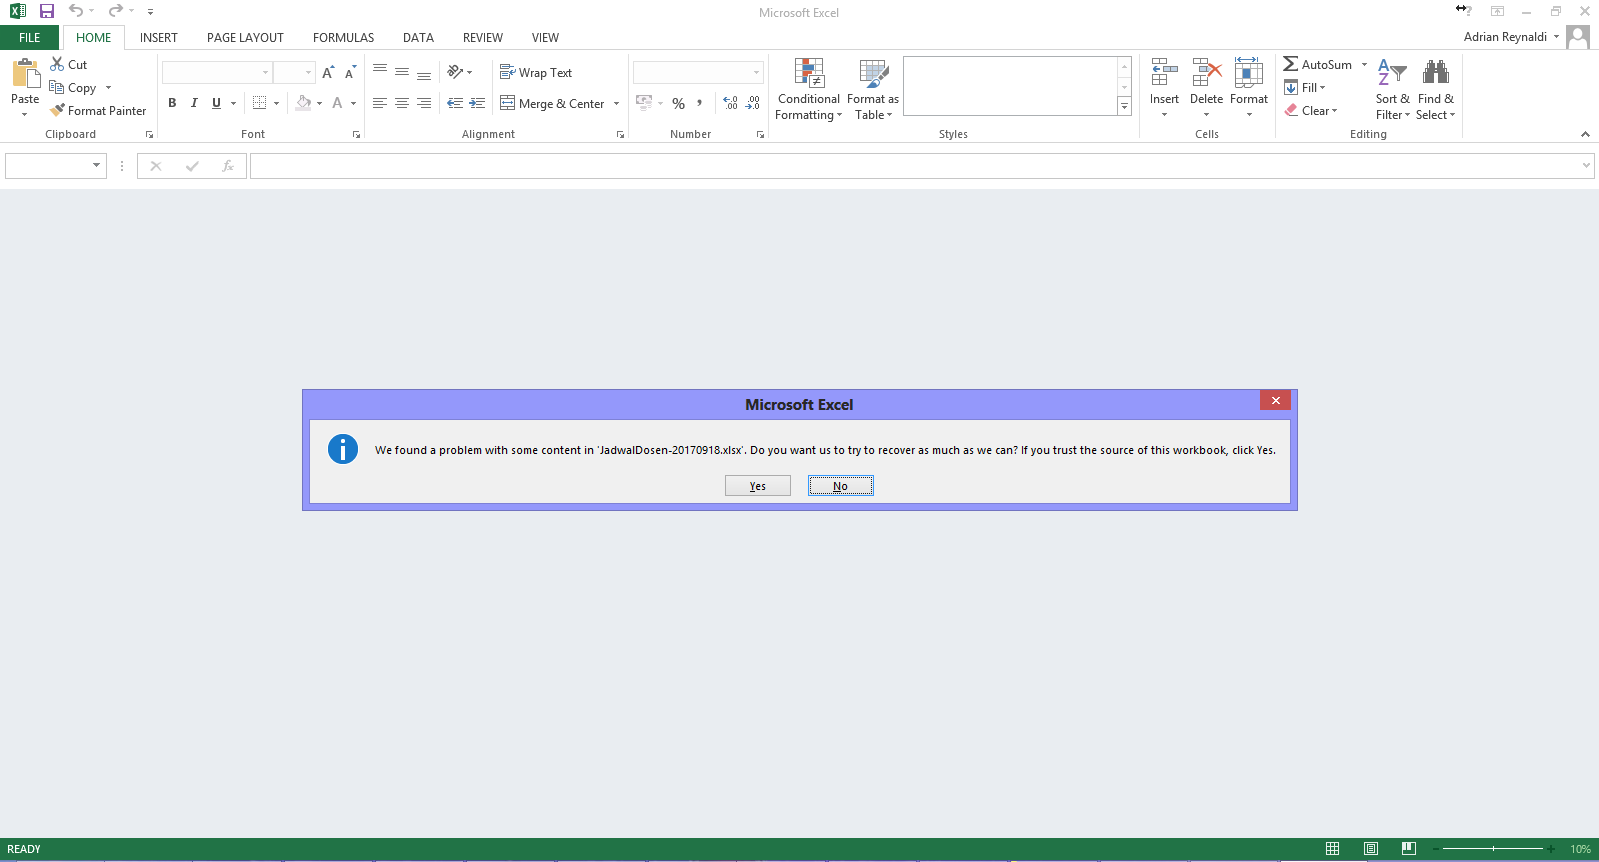
\includegraphics[scale=0.4]{erorXLSX.png}}
	\caption[Tampilan eror saat membuka file bertipe .xlsx]{Tampilan eror saat membuka file bertipe .xlsx} 
	\label{fig:flow-chart-CodeIgniter} 
\end{figure}

\begin{figure} [H]
	\centering  
	\frame{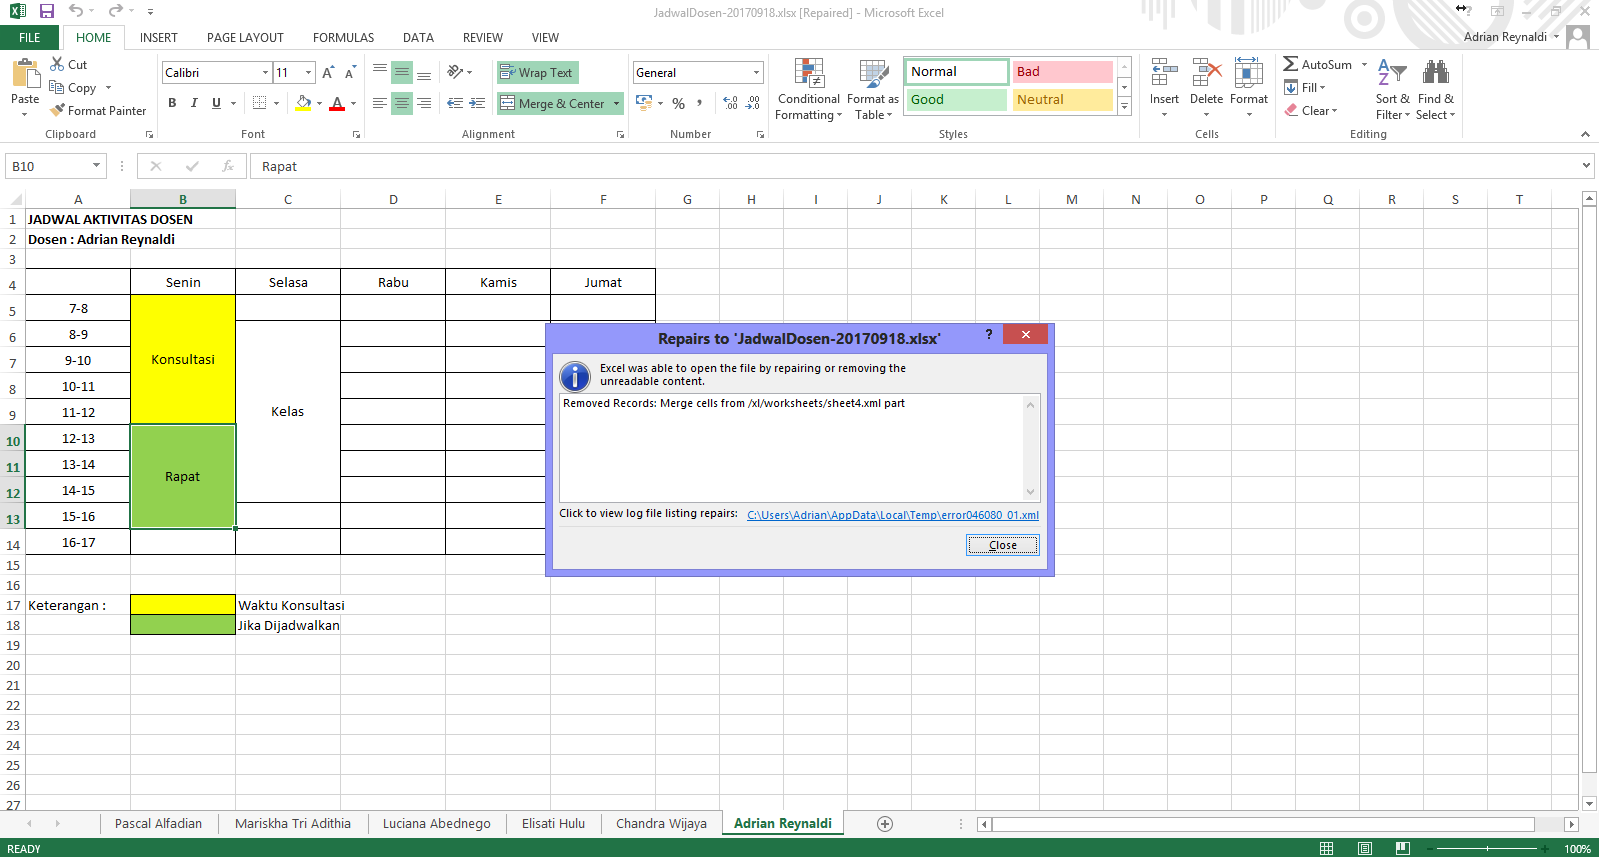
\includegraphics[scale=0.4]{erorXLSXDetail.png}}
	\caption[Keterangan Eror File .xlsx]{Keterangan Eror File .xlsx} 
	\label{fig:flow-chart-CodeIgniter} 
\end{figure}

Log eror:
\begin{lstlisting}
<?xml version="1.0" encoding="UTF-8" standalone="yes"?>
<recoveryLog xmlns="http://schemas.openxmlformats.org/spreadsheetml/2006/main">
<logFileName>error046080_01.xml</logFileName>
<summary>Errors were detected in file 'C:\Users\Adrian\Documents\Tugas\Skripsi\XLS Testing\JadwalDosen-20170918.xlsx'</summary>
<removedRecords summary="Following is a list of removed records:"><removedRecord>Removed Records: Merge cells from /xl/worksheets/sheet4.xml part
</removedRecord></removedRecords></recoveryLog>
\end{lstlisting}
\paragraph{}Dilihat dari log eror tersebut, eror ini terjadi karena ada perintah \textit{merge cells} yang dihapus oleh MS Excel. Hal ini terjadi karena adanya perintah dari PHPExcel versi 1.8.0 yang belum mendukung file bertipe .xlsx.
\paragraph{}Karena eror di atas disebabkan oleh permasalahan kompabilitas PHPExcel 1.8.0 dan tipe file .xlsx, maka hal ini dapat diatasi dengan cara mengubah tipe file yang diekspor dari file .xlsx menjadi tipe yang lebih lama yaitu .xls.
\newline
\newline
Potongan kode lama yang menyebabkan eror:
\begin{lstlisting}
 $filename = 'JadwalDosen-'.date("Ymd").'.xlsx'; //Nama file XLS yang akan dibuat
 header('Content-type: application/vnd.ms-excel');
 header('Content-Disposition: attachment;filename="' . $filename . '"');

 $objWriter = PHPExcel_IOFactory::createWriter($this->excel, 'Excel2007');
\end{lstlisting}
Potongan kode baru untuk menghilangkan eror:
\begin{lstlisting}
 $filename = 'JadwalDosen-'.date("Ymd").'.xls'; //Nama file XLS yang akan dibuat
 header('Content-type: application/vnd.ms-excel');
 header('Content-Disposition: attachment;filename="' . $filename . '"');

 $objWriter = PHPExcel_IOFactory::createWriter($this->excel, 'Excel5');
\end{lstlisting}
Seperti bisa dilihat pada dua potongan kode program di atas, terjadi perubahan pada baris pertama kode dan baris terakhir kode. Pada baris pertama ekstensi file diubah dari .xlsx menjadi .xls. Pada baris terakhir tipe spreadsheet diubah dari 'Excel2007' menjadi 'Excel5'.
\paragraph{}Setelah tipe file diubah menjadi  .xls, eror di Microsoft Excel pun hilang.
\begin{figure} [H]
	\centering  
	\frame{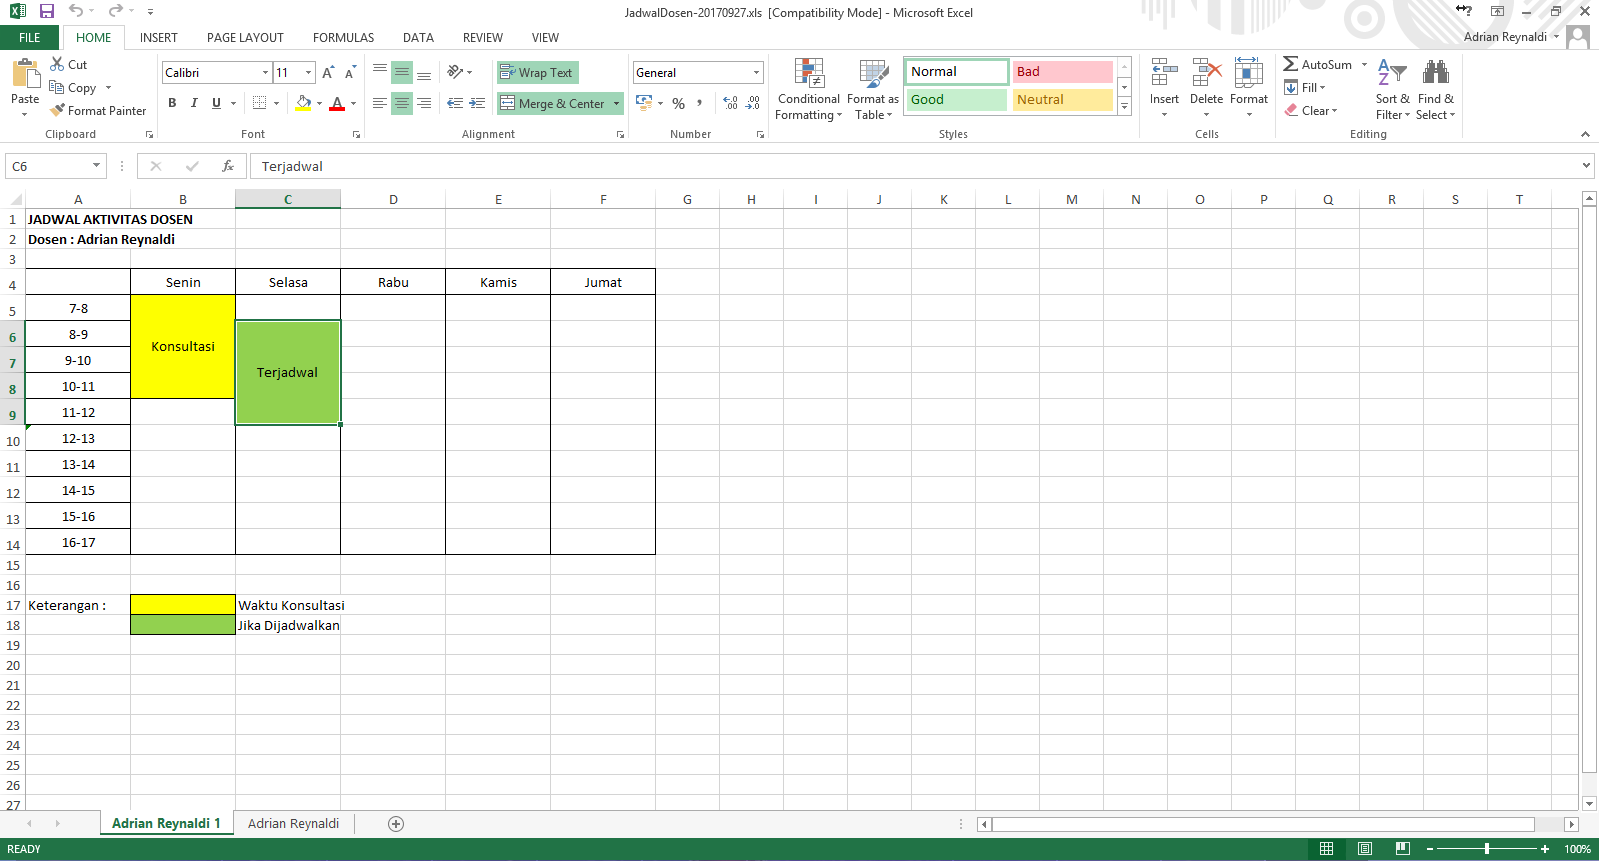
\includegraphics[scale=0.4]{tesXLSSukses.png}}
	\caption[Eror Sudah Tidak Muncul Ketika File Dibuka]{Eror Sudah Tidak Muncul Ketika File Dibuka} 
	\label{fig:eror-hilang} 
\end{figure}

\subsection{Pengujian Eksperimental Penambahan Tombol \textit{Delete All}}
Tombol "Delete All" berfungsi untuk menghapus semua jadwal yang sudah dimasukan oleh pengguna. Hasil yang diharapkan adalah ketika tombol ini ditekan akan memunculkan pop-up dan ketika tombol "ok" ditekan akan mengeksekusi perintah untuk menghapus semua jadwal milik user.
\subsubsection{Hasil Pengujian}
Tombol "Delete All" dibuat di halaman EntriJadwalDosen di pojok kiri bawah.
\begin{figure} [H]
	\centering  
	\frame{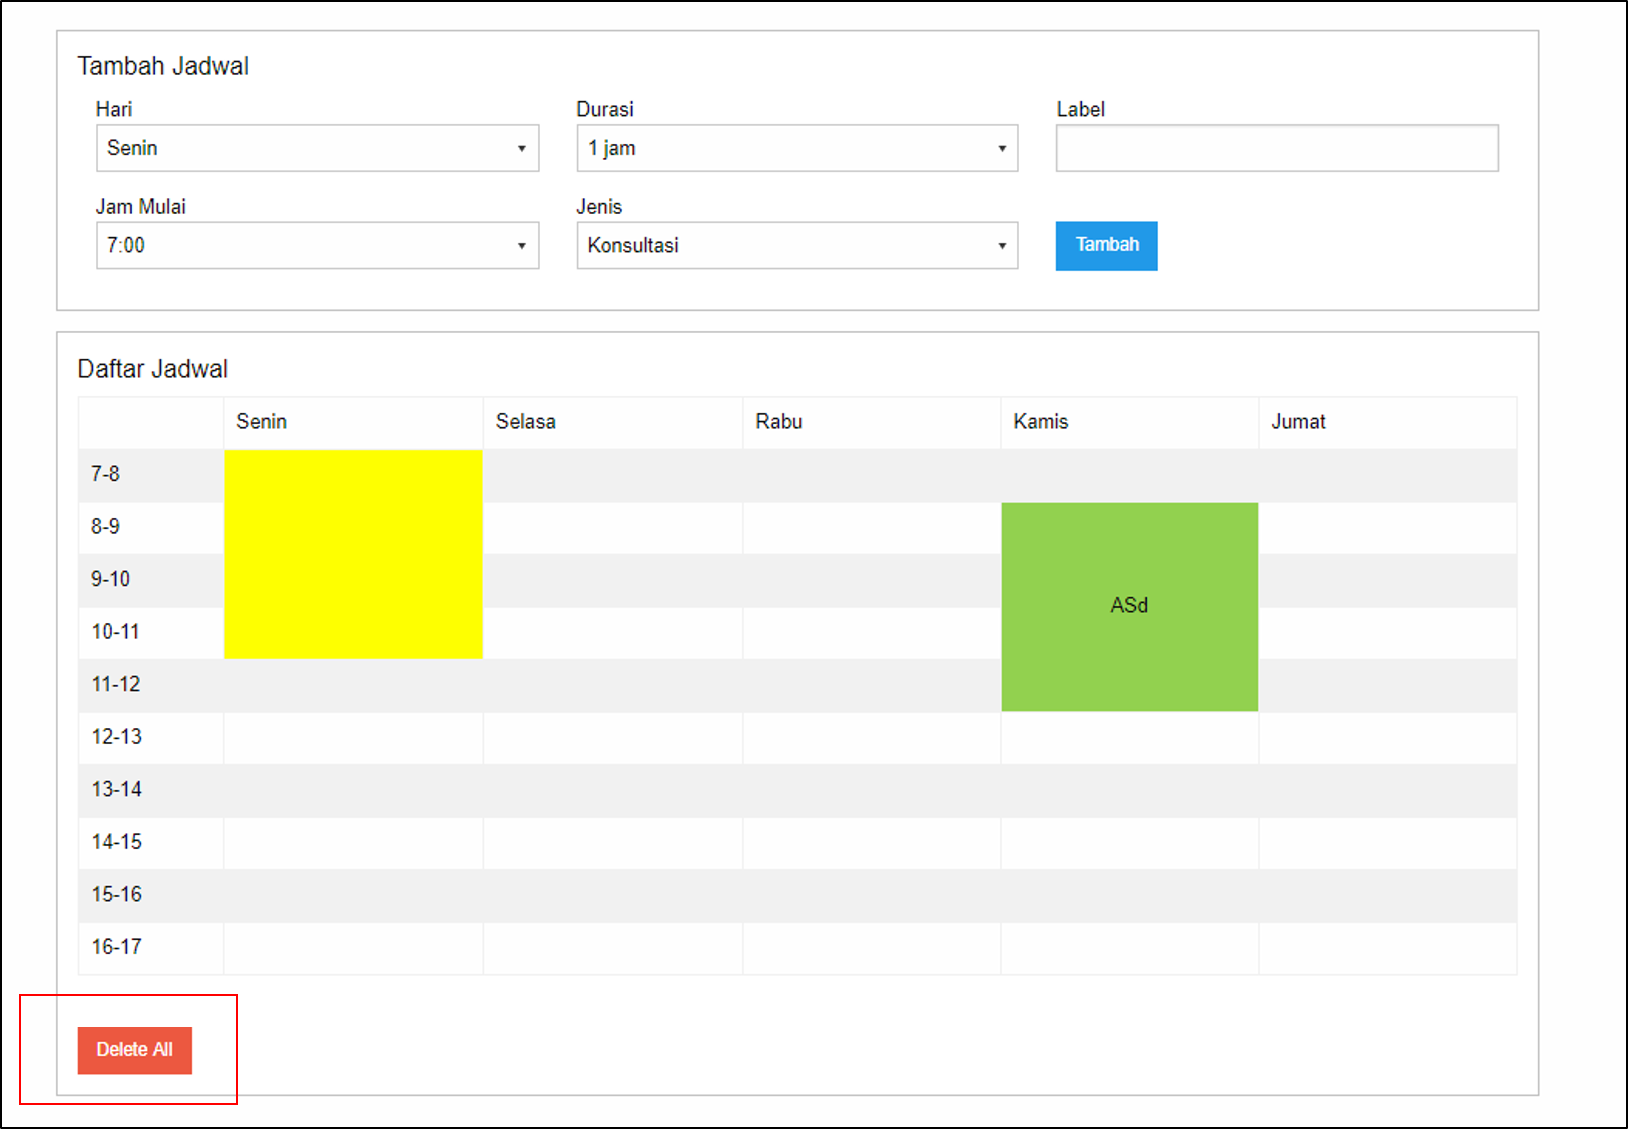
\includegraphics[scale=0.5]{deleteAllButton.png}}
	\caption[Tombol \textit{Delete All} di Entri Jadwal Dosen]{Tombol \textit{Delete All} di Entri Jadwal Dosen} 
	\label{fig:flow-chart-CodeIgniter} 
\end{figure}
Ketika tombol "Delete All" ditekan muncul tampilan konfirmasi
\begin{figure} [H]
	\centering  
	\frame{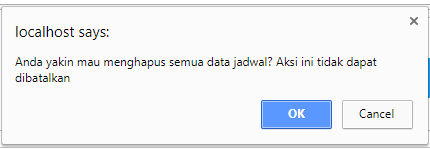
\includegraphics[scale=0.5]{popupDeleteAll.png}}
	\caption[Tampilan Konfirmasi]{\textbf{Tombol \textit{Delete All} di Entri Jadwal Dosen}} 
	\label{fig:flow-chart-CodeIgniter} 
\end{figure}
Setelah tombol "ok" ditekan, semua jadwal dihapus
\begin{figure} [H]
	\centering  
	\frame{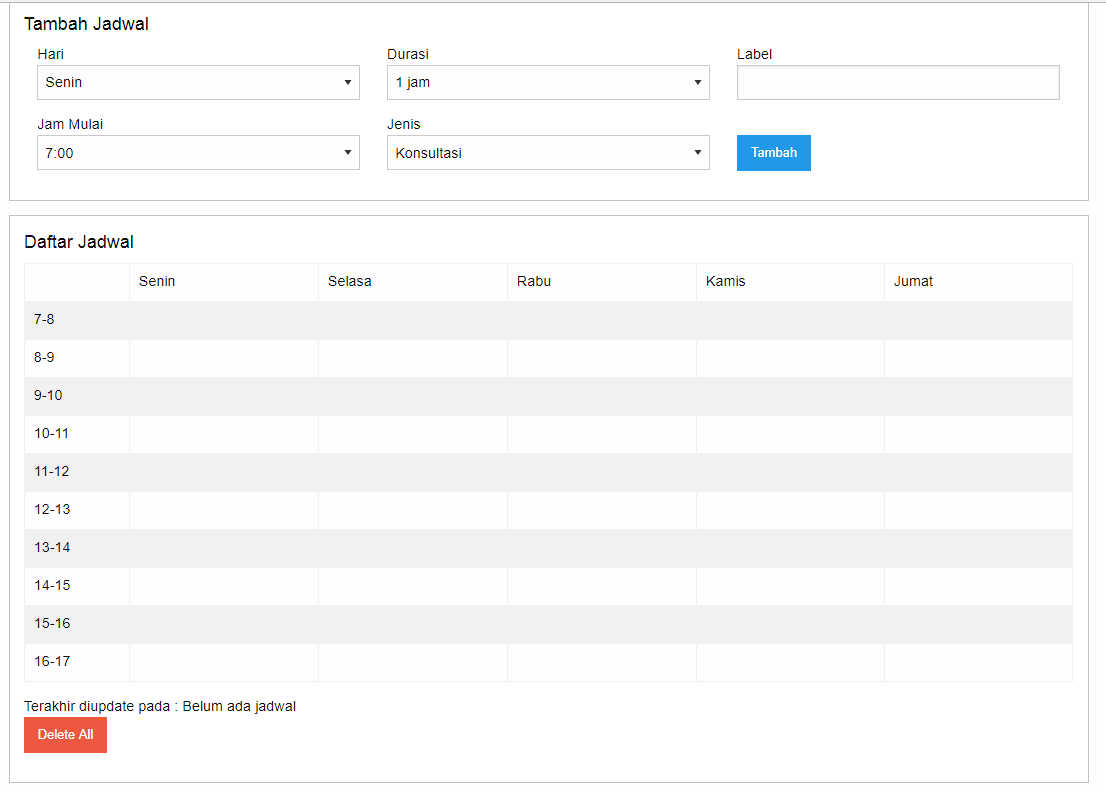
\includegraphics[scale=0.5]{empty.png}}
	\caption[Semua Jadwal Dihapus]{Semua Jadwal Dihapus} 
	\label{fig:flow-chart-CodeIgniter} 
\end{figure}
Hasil pengujian berjalan lancar dan sesuai dengan hasil yang diharapkan.

\subsection{Pengujian Eksperimental Penambahan Informasi Waktu \textit{Update} Terakhir Jadwal}
Informasi waktu \textit{update} terakhir jadwal oleh pengguna berfungsi agar pengguna dapat membedakan apakah jadwal miliknya merupakan versi lama yang sudah tidak dipakai atau merupakan versi baru. Hasil yang diharapkan adalah muncul label di halaman EntriJadwalDosen dan LihatJadwalDosen.
\subsubsection{Hasil Pengujian}
Label berisi tanggal terakhir update jadwal muncul di halaman EntriJadwalDosen
\begin{figure} [H]
	\centering  
	\frame{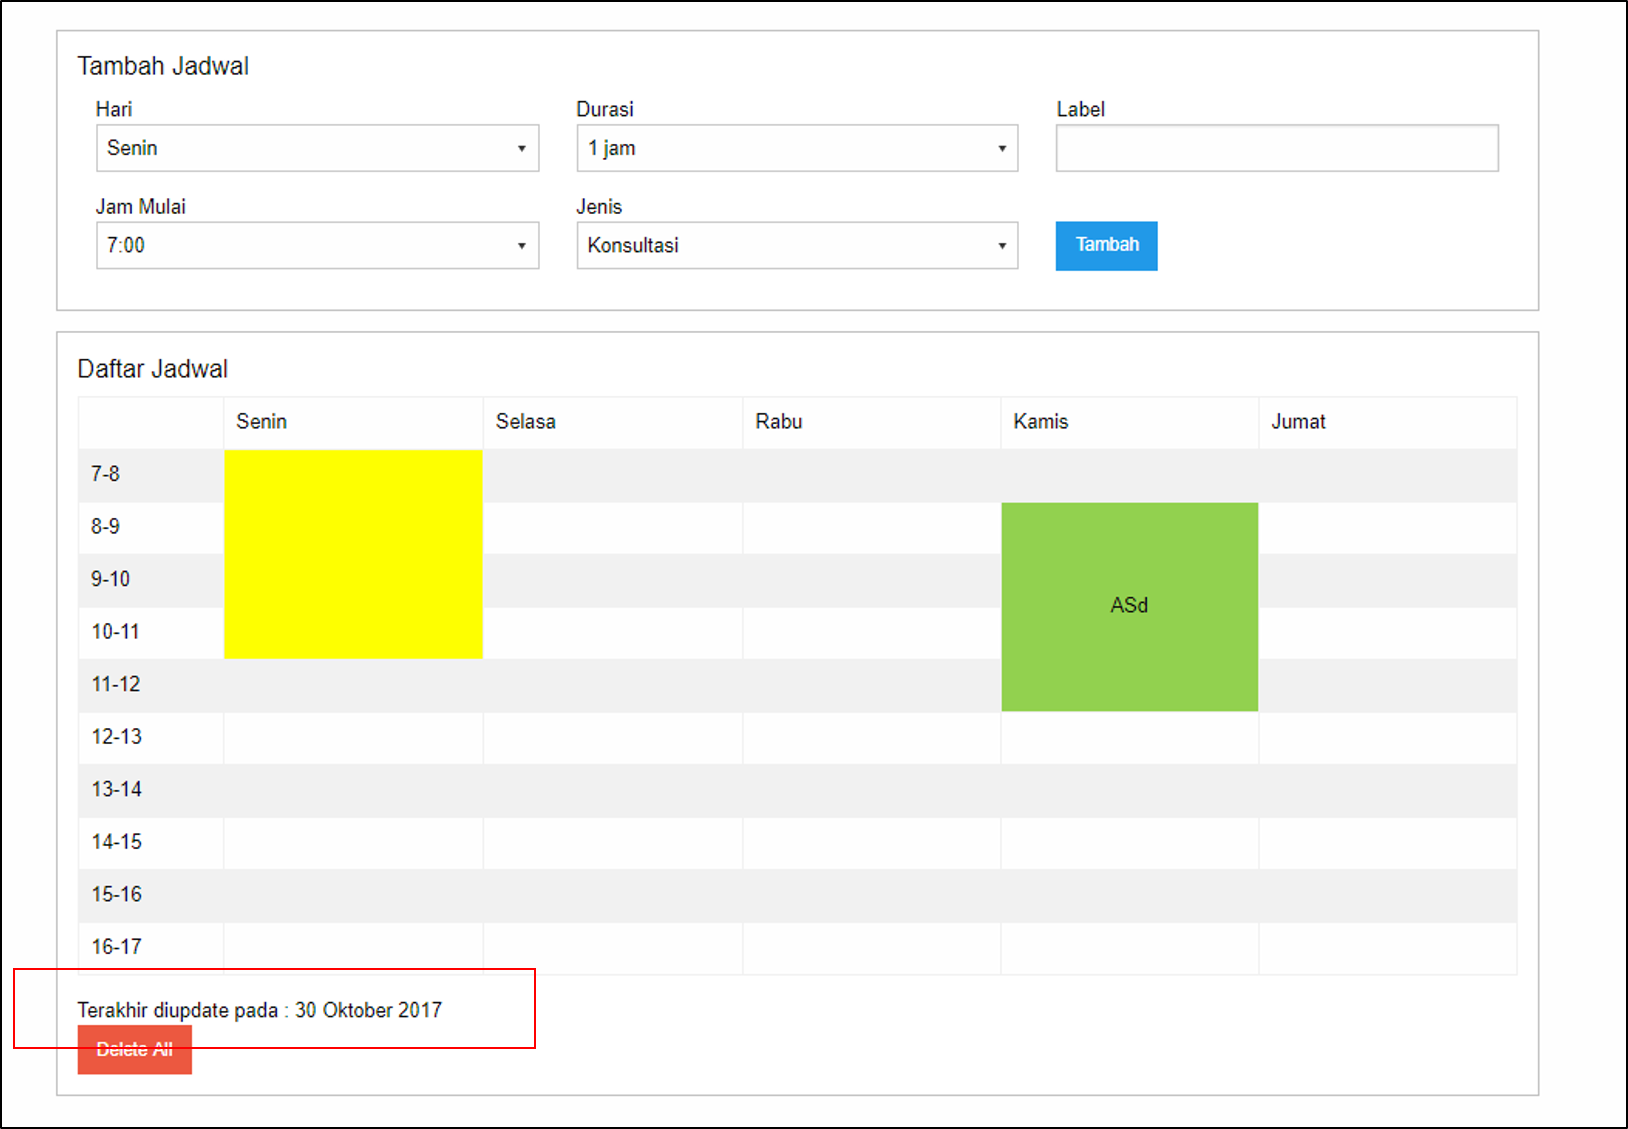
\includegraphics[scale=0.5]{updateTerakhir.png}}
	\caption[Informasi Waktu \textit{Update} Terakhir Jadwal di Entri Jadwal Dosen]{Informasi Waktu \textit{Update} Terakhir Jadwal di Entri Jadwal Dosen} 
	\label{fig:flow-chart-CodeIgniter} 
\end{figure}
Label berisi tanggal terakhir update jadwal muncul di halaman LihatJadwalDosen
\begin{figure} [H]
	\centering  
	\frame{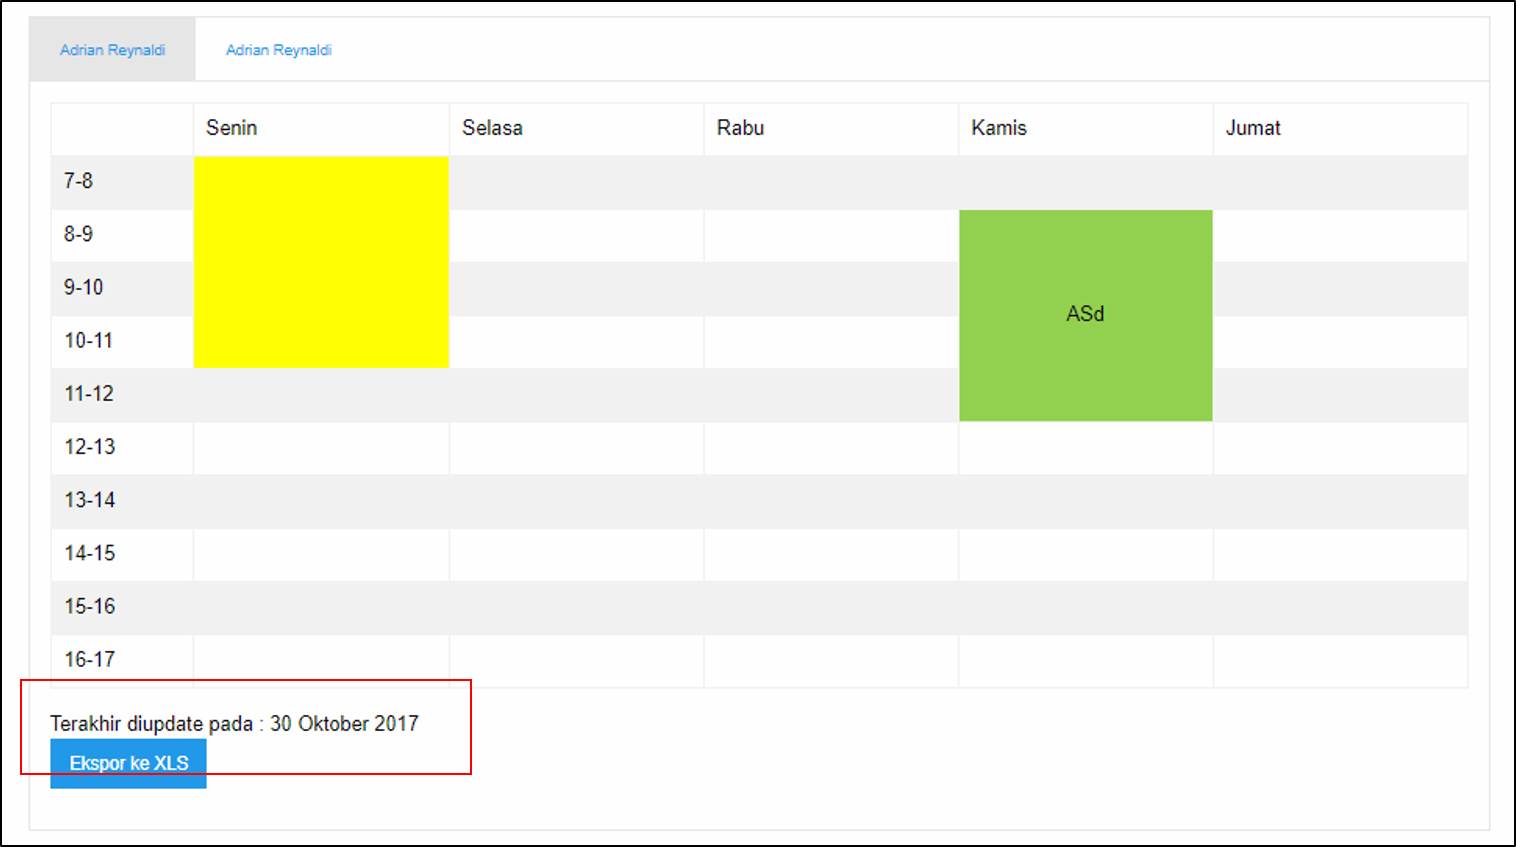
\includegraphics[scale=0.5]{updateTerakhirLihat.png}}
	\caption[Informasi Waktu \textit{Update} Terakhir Jadwal di Lihat Jadwal Dosen]{Informasi Waktu \textit{Update} Terakhir Jadwal di Lihat Jadwal Dosen} 
	\label{fig:flow-chart-CodeIgniter} 
\end{figure}
Hasil pengujian berjalan lancar dan sesuai dengan hasil yang diharapkan.